\documentclass[a4paper,10pt]{article}
\usepackage[utf8]{inputenc}
\usepackage{graphicx}
\usepackage{hyperref}
\usepackage{dirtree}
\usepackage{listings}
\newcommand\tab[1][1cm]{\hspace*{#1}}
\title{Técnicas de Búsqueda con Adversarios\\(4ª semana)}
\begin{document}
\maketitle
\pagebreak
\graphicspath{/mnt/data_1/code/asignaturas/sint/practicas/pr3}
\section{Ejercicio 1}
\subsection{Enunciado}
Sea un grafo con coeficiente de ramificacion 3, simetrico y cuya profundidad es 3:\\
nombraremos sus nodos de la sigiente manera:\\
\dirtree{%
.1 0.
.2 1().
.3 1.1().
.4 1.1.1(8).
.4 1.1.2(7).
.4 1.1.3(3).
.3 1.2().
.4 1.2.1(9).
.4 1.2.2(1).
.4 1.2.3(6).
.3 1.3().
.4 1.3.1(2).
.4 1.3.2(4).
.4 1.3.3(1).
.2 2().
.3 2.1().
.4 2.1.1(1).
.4 2.1.2(3).
.4 2.1.3(5).
.3 2.2().
.4 2.2.1(3).
.4 2.2.2(9).
.4 2.2.3(2).
.3 2.3().
.4 2.3.1(6).
.4 2.3.2(5).
.4 2.3.3(2).
.2 3().
.3 3.1().
.4 3.1.1(1).
.4 3.1.2(2).
.4 3.1.3(3).
.3 3.2().
.4 3.2.1(9).
.4 3.2.2(7).
.4 3.2.3(2).
.3 3.3().
.4 3.3.1(16).
.4 3.3.2(6).
.4 3.3.3(4).
}
\vspace{0.5cm}
Se obia que todos son descendientes de el nodo 0\\
La poda alfa beta seria de la siguiente forma (resuelta en el propio libro de problemas)\\
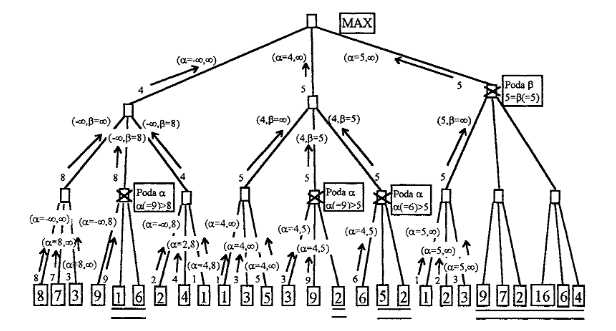
\includegraphics[scale=0.8]{poda_alfa_beta.png}
\vspace{1cm}
\\A continuación aplicaremos el minmax sin poda alfa poda, donde [x] representa la iteración
\\el orden de elecion es el siguiente:
\dirtree{%
.1 max.
.2 min.
.3 max.
.4 fin.
}
\dirtree{%
.1 0(5)[12].
.2 1(4)[3].
.3 1.1(8)[0].
.4 1.1.1(8).
.4 1.1.2(7).
.4 1.1.3(3).
.3 1.2(9)[1].
.4 1.2.1(9).
.4 1.2.2(1).
.4 1.2.3(6).
.3 1.3(4)[2].
.4 1.3.1(2).
.4 1.3.2(4).
.4 1.3.3(1).
.2 2(5)[7].
.3 2.1(5)[4].
.4 2.1.1(1).
.4 2.1.2(3).
.4 2.1.3(5).
.3 2.2(9)[5].
.4 2.2.1(3).
.4 2.2.2(9).
.4 2.2.3(2).
.3 2.3(6)[6].
.4 2.3.1(6).
.4 2.3.2(5).
.4 2.3.3(2).
.2 3(3)[11].
.3 3.1(3)[8].
.4 3.1.1(1).
.4 3.1.2(2).
.4 3.1.3(3).
.3 3.2(9)[9].
.4 3.2.1(9).
.4 3.2.2(7).
.4 3.2.3(2).
.3 3.3(16)[10].
.4 3.3.1(16).
.4 3.3.2(6).
.4 3.3.3(4).
}
\vspace{1cm}
Siendo el recorrido final:
\vspace{1cm}
\dirtree{%
.1 0(5)[12] max.
.2 2(5)[7] min.
.3 2.1(5)[4] max.
.4 2.1.3(5) end.
}
\pagebreak
\section{Problema de las comidas}
\subsection{Enunciado}
\vspace{0.1cm}
Resuelve el siguiente problema tanto por minimax como poda alfa-beta, añadiendo junto a cada nodo la información como se indica en el apartado anterior.
Tu hermano mayor y tú, vais a cenar. Vuestra madre ha preparado dos platos: coles de bruselas y brócoli, y os ha dicho que os lo comáis todo. Decidís que os vais a repartir los platos de la siguiente forma: primero, tú eliges entre comer uno de los dos platos o echarte la mitad de uno de ellos; después, tu hermano puede realizar las mismas elecciones sobre lo que quede en la mesa; así, mientras quede algo en la mesa, os iréis alternando en la elecciones (según este esquema, puede que alguno acabe comiendo más comida que el otro). Tú has cometido el error de hacerle saber tus preferencias a tu hermano, que son las que se muestran en la siguiente tabla. Sabiendo que el objetivo de tu hermano es únicamente fastidiarte, ¿qué plato debes elegir primero?
\dirtree{%
.1 0[]().
.2 1[]().
.3 1.1[](0) <b>.
.3 1.2[]().
.4 1.2.1[](-5) <b+c/2>.
.2 2[]().
.3 2.1[](-10) <c>.
.3 2.2[]().
.4 2.2.1[](-15) <c+b/2>.
.2 3[]().
.3 3.1[]().
.4 3.1.1[](0) <b>.
.3 3.2[]().
.4 3.2.1[]().
.5 3.2.1.1[](+5) <c/2+b/2>.
.4 3.2.2[]().
.5 3.2.2.1[](0) <b>.
.3 3.3[]().
.4 3.3.1[](-15) <c+b/2>.
.4 3.3.2[]().
.5 3.3.2.1[](+5) <c/2+b/2>.
.2 4[]().
.3 4.1[]().
.4 4.1.1[](-10) <c>.
.3 4.2[]().
.4 4.2.1[]().
.5 4.2.1.1[](-10) <c>.
.4 4.2.2[]().
.5 4.2.2.1[](+5) <c/2+b/2>.
.3 4.3[]().
.4 4.3.1[](-5) <b+c/2>.
.4 4.3.2[]().
.5 4.3.2.1[](+5) <c/2+b/2>.
}
\pagebreak
El anterior grafo indica los estados finales (sin las desiciones intermedias) de este problema.\\
Así pues aplicaremos minmax y minmax con poda alfa beta
\dirtree{%
.1 max (2).
.2 min (3).
.3 max (4).
.4 min (5).
.5 max (6).
}
\subsection{minmax}
\dirtree{%
.1 0[15](-15).
.2 1[2](-5).
.3 1.1[1](0) <b>.
.3 1.2[2](-5).
.4 1.2.1[2](-5) <b+c/2>.
.2 2[4](-15).
.3 2.1[3](-10) <c>.
.3 2.2[4]().
.4 2.2.1[4](-15) <c+b/2>.
.2 3[5](0).
.3 3.1[5](0).
.4 3.1.1[5](0) <b>.
.3 3.2[6](+5).
.4 3.2.1[6](+5).
.5 3.2.1.1[6](+5) <c/2+b/2>.
.4 3.2.2[7](0).
.5 3.2.2.1[7](0) <b>.
.3 3.3[8](-15).
.4 3.3.1[8](-15) <c+b/2>.
.4 3.3.2[9](+5).
.5 3.3.2.1[9](+5) <c/2+b/2>.
.2 4[10](-10).
.3 4.1[10](-10).
.4 4.1.1[10](-10) <c>.
.3 4.2[12](+5).
.4 4.2.1[11](-10).
.5 4.2.1.1[11](-10) <c>.
.4 4.2.2[12](+5).
.5 4.2.2.1[12](+5) <c/2+b/2>.
.3 4.3[14](+5).
.4 4.3.1[13](-5) <b+c/2>.
.4 4.3.2[14](+5).
.5 4.3.2.1[14](+5) <c/2+b/2>.
}
\pagebreak
\subsection{Poda alfa beta}
\dirtree{%
.1 0[4](-15).
.2 1[2](-5).
.3 1.1[1](0) <b>.
.3 1.2[2](-5).
.4 1.2.1[2](-5) <b+c/2>.
.2 2[4](-15).
.3 2.1[3](-10) <c>.
.3 2.2[4](-15).
.4 2.2.1[4](-15) <c+b/2>.
.2 3[5](0).
.3 3.1[5](0).
.4 3.1.1[5](0) <b>.
.3 3.2[6](+5).
.4 3.2.1[6](+5).
.5 3.2.1.1[6](+5) <c/2+b/2>.
.4 3.2.2[]() no eplorada.
.5 3.2.2.1[](0) <b> no eplorada.
.3 3.3[8](+5).
.4 3.3.1[7](-15) <c+b/2>.
.4 3.3.2[8](+5).
.5 3.3.2.1[8](+5) <c/2+b/2>.
.2 4[9](-10).
.3 4.1[9](-10).
.4 4.1.1[9](-10) <c>.
.3 4.2[11](+5).
.4 4.2.1[10](-10).
.5 4.2.1.1[10](-10) <c>.
.4 4.2.2[11](+5).
.5 4.2.2.1[11](+5) <c/2+b/2>.
.3 4.3[12](-5).
.4 4.3.1[12](-5) <b+c/2>.
.4 4.3.2[]() no eplorada.
.5 4.3.2.1[](+5) <c/2+b/2> no eplorada.
}

\vspace*{\fill}
\raggedleft Documento escrito en \LaTeX{}
\end{document}
